\chapter{Implementation}

In this section the general approach is described, aswell as trial and error. One must keep in mind that steps have been boiled down to the most notable. Also all the different tools that were used where expanded as time passed, certainly not all packages and software are required for all steps but where helpfull in building, compiling, flashing and auxillary tasks. 

\section{Work Environment}\label{envsetup.ch}
To provide a portable environment where source code, different tools and toolchains can be placed, a docker container was created. The main advantages of Docker are that tools such as Buildroot \ref{buildroot.ch}, qemu, toolchains, etc are available on Linux. With the additional benefit of the possibilty to automate large parts of the compilation processes through shell scripts, and potentially out sourcing expensiv compilation, in the absence of capable local hardware, to the cloud, Docker seems to be a good fit.

To build a Docker container from an image the Dockerfile is specified in [...........]. The official Ubuntu 20.04 long time support (LTS) baseimage is used. This provides a solid OS with many tools that facilitate aquiering packages with the included packet manager \code{apt-get}. 

A lot of different To install debendencies the installscript.sh is run automatically when building the image. This script includes a variety of different packages that will be required. A set of basic tools enables working inside the container on a CLI, a collection of the most common and broadly used untilies are shown in listing \ref{basic-util}. We use \code{git} and \code{wget} to aquire repositories and files from the internet, a CLI text editor for \code{.config} files, and compressing and uncompressing utility. Any scripts that are displayed, unless specifically stated otherwise, work with the \code{bash} shell.

\begin{lstlisting}[style=SH, caption=Installing basic utility, label=basic-util, float, floatplacement=H]
apt-get install -y git \
wget \
bc \
nano \
curl \
cpio \
unzip \
rsync
\end{lstlisting}

To be able to cross-compile source code to architectures specific binaries for the target device we require further packages, all of which are available on Ubuntu's package manager \code{apt-get}.

\begin{lstlisting}[style=SH, caption=Installing toolchains and dependencies, label=toolchain-util, float, floatplacement=H]
apt-get install -y gcc \
binutils-arm-none-eabi \
make \
gcc-arm-none-eabi \
gcc-arm-linux-gnueabihf \
gcc-arm-linux-gnueabi \
libncurses-dev \
libncurses5-dev \
flex \
bison \
openssl \
libssl-dev \
dkms \
perl \
libelf-dev \
libudev-dev \
libpci-dev \
libiberty-dev \
autoconf \
lzop 
\end{lstlisting}

\section{Sample Code}

To establish a baseline with less complex code compared to the massive source code repepository of the Linux kernel, and all its forks, that can fully be understood, a collection of sample code was found~\cite{sample-code}. These three code snippets, in combination with QEMU as an emulator for target platform, will provide a controlled environment, in which it is easier to verify if compilation was successful and correct, if the binaries works on target platform, or if it was correctly linked. By having such a fall back option it saves  time and power, and provides a solid foundation of the complex processes that occur during cross-compilation. 

\code{notmain.c}, as seen in listing \ref{lst:notmain.c}, writen in the C programming language represents the kernel, which contains the basic loop, with the task of printing the numbers 0 to 7 onto some universal asynchronous receiver-transmitter (UART). Theoretically, if the UART is connected to some console, the output would look something like this:

\code{01234567}

\begin{lstlisting}[style=CEE, caption={notmain.c}\label{lst:notmain.c}, float, floatplacement=H]
void PUT32 ( unsigned int, unsigned int );
#define UART0BASE 0x4000C000
int notmain ( void )
{
    unsigned int rx;
    for(rx=0;rx<8;rx++)
    {
        PUT32(UART0BASE+0x00,0x30+(rx&7));
    }
    return(0);
}
\end{lstlisting}

\begin{lstlisting}[style=ASS, caption={flash.s}, float, floatplacement=H]
.thumb
.thumb_func
.global _start
_start:
stacktop: .word 0x20001000
.word reset
.word hang

.thumb_func
reset:
    bl notmain
    b hang

.thumb_func
hang:   b .

.thumb_func
.globl PUT32
PUT32:
    str r1,[r0]
    bx lr
\end{lstlisting}

\begin{lstlisting}[style=LD, caption={flash.ld}, float, floatplacement=H]
ENTRY(_start)

MEMORY
{
    rom : ORIGIN = 0x00000000, LENGTH = 0x1000
    ram : ORIGIN = 0x20000000, LENGTH = 0x1000
}

SECTIONS
{
    .text : { *(.text*) } > rom
    .rodata : { *(.rodata*) } > rom
    .bss : { *(.bss*) } > ram
}
\end{lstlisting}

To compile this sample code for target platfrom the commands shown in listing \ref{compSample} are issued through the command line shell \code{bash}. Initially starting with three files \code{flash.s}, \code{notmain.c} and \code{flash.ld}, we are now presented with 5 additional files. \code{flash.o}, \code{notmain.o}, \code{notmain.elf}, \code{notmain.list} and most importantly \code{notmain.bin}, the "sample kernel". From listing \ref{compSample} we can also see the flag \code{-mcpu=cortex-m4}, symbolizing that we are compiling for target platfrom ARM Cortex-M4.

\begin{lstlisting}[style=SH, caption=Compiling sample code with gcc-arm-none-eabi toolchain, label=compSample, float, floatplacement=H]
arm-none-eabi-as --warn --fatal-warnings -mcpu=cortex-m4 flash.s -o flash.o
arm-none-eabi-gcc -Wall -O2 -ffreestanding -mcpu=cortex-m4 -mthumb -c notmain.c -o notmain.o
arm-none-eabi-ld -nostdlib -nostartfiles -T flash.ld flash.o notmain.o -o notmain.elf
arm-none-eabi-objdump -D notmain.elf > notmain.list
arm-none-eabi-objcopy -O binary notmain.elf notmain.bin
\end{lstlisting}

\section{Compilation}

\subsection{U-Boot}
As a first step, we will compile U-Boot for QEMU, so that we can continue evaluating, without needing to flash onto an MCU every time. If not previously done so, we need to clone the U-Boot repository, and navigate inside the freshly cloned folder. Using our previously established toolchain, \code{gcc-arm-none-eabi}, we call the commands, shown in listing \ref{compQEMUuboot}, inside of the current folder. At line 2 of listing \ref{compQEMUuboot}, \code{qemu\_arm\_defconfig}, is mentioned after having declared the toolchain. This config is simply a pre-set configuration file that is provided by U-Boot, for specific usecases. After compilation has completed \code{u-boot.bin} is the output of our compilation.

\begin{lstlisting}[style=SH, caption=Compiling U-Boot for QEMU, label=compQEMUuboot]
make mrproper
make ARCH=arm CROSS_COMPILE=arm-none-eabi- qemu_arm_defconfig
make ARCH=arm CROSS_COMPILE=arm-none-eabi-
\end{lstlisting}

\begin{lstlisting}[style=SH, caption=Compiling U-Boot for QEMU, label=compQEMUuboot]
make stm32f469_disco_sd_defconfig
make
\end{lstlisting}

\subsection{Mainline Linux kernel}

[I did this but its pretty pointless, idk. the explorative nature of this thesis had me running against a lot of walls and IDK how to show that. I mean with buildroot, that was found lateron in the thesis, things work easier, but this work here seems to be for nothing.]

\subsection{$\mu$Clinux}

[I did this but its pretty pointless, idk. the explorative nature of this thesis had me running against a lot of walls and IDK how to show that. I mean with buildroot, that was found lateron in the thesis, things work easier, but this work here seems to be for nothing.]


\subsection{Buildroot}
We need to download and navigate to the buildroot directory. In the documentation of Buildroot, under 2.1. "Mandatory packages", a list of required dependencies for the compilation process are shown, we have installed some of these packages in section \ref{envsetup.ch}, and others come with the Ubuntu 20.04 LTS distribution. We are presented with the build root directory shown in listing \ref{buildrootdir}. \code{configs} holds all the pre-set configuration files that can be used to compile Linux, by navigating to the directory we see all the configs that can be used, and lateron modified. Sadly STM32L476G-Eval is not included, but other configurations for STM are available, such as \code{stm32f429\_disco\_xip\_defconfig} for the STM32F429-Discovery development board. \code{make stm32f429\_disco\_xip\_defconfig} will copy the code from the specified configuration into the \code{.config} file, which is not visible in the thee unless command \code{ls -a} is issued. 

\begin{lstlisting}[caption=Buildroot directory, label=buildrootdir]
buildroot/
|
|-- arch
|-- board
|-- boot
|-- configs
|-- docs
|-- linux
|-- package
|-- support
|-- system
|-- toolchain
|-- utils
\end{lstlisting}

Seen in \ref{fig:buildroot-menuconfig}, by typing \code{make menuconfig} will open a visual menu inside the console that can help us visually navigate through the \code{.config} file that was previously set. Note that for this visual editor the \code{libncurses5-dev} package is required and was installed in section \ref{envsetup.ch}.

\begin{figure}
\centering
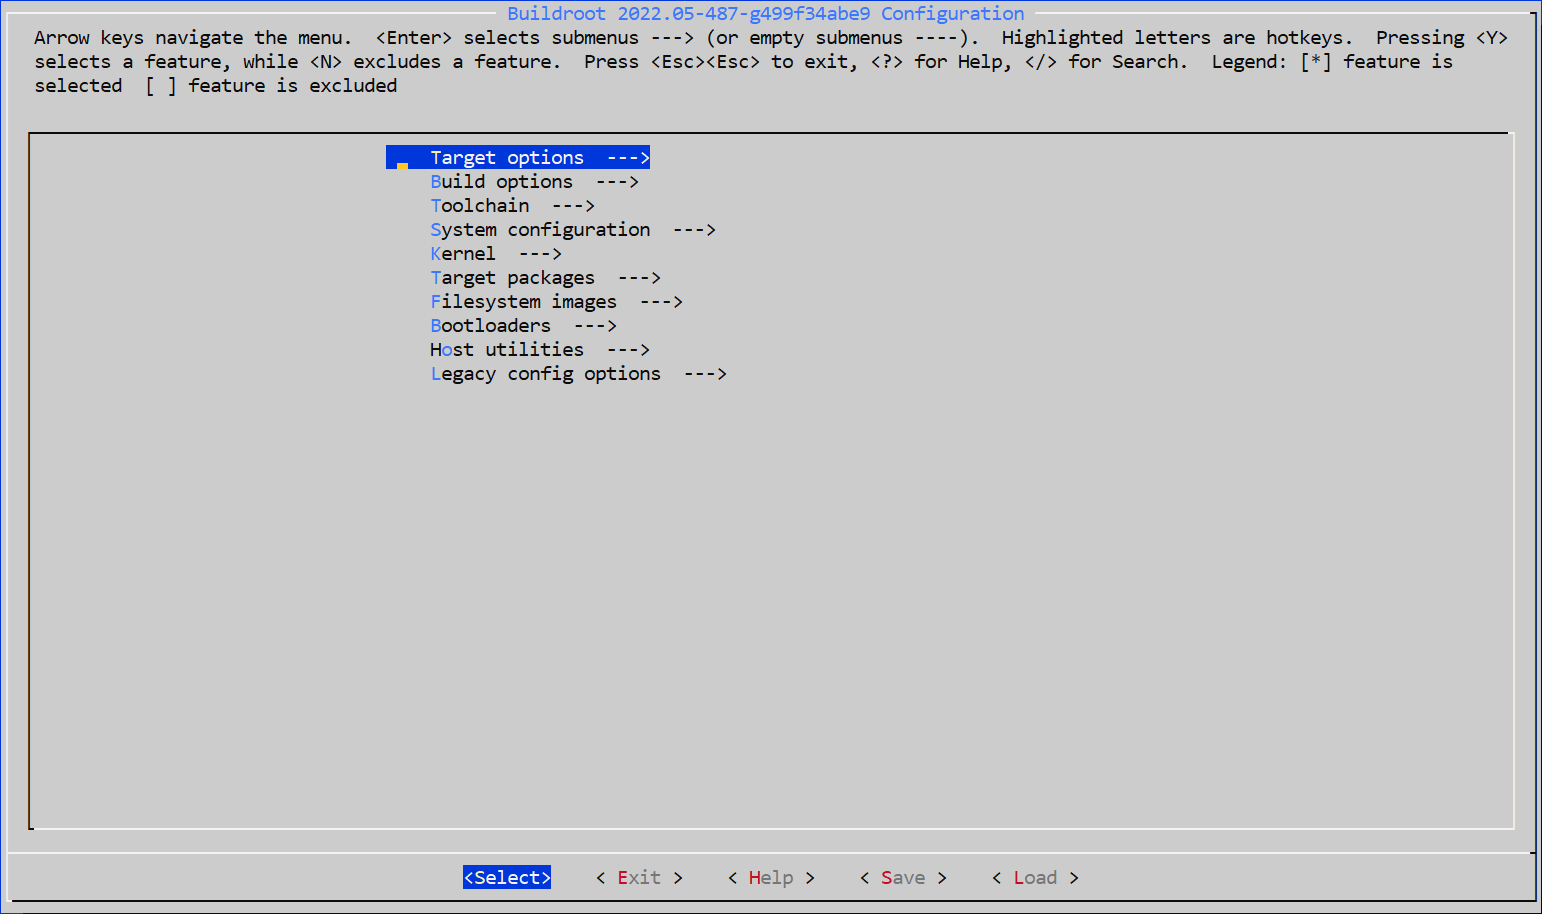
\includegraphics[width=0.6\textwidth]{buildroot-menuconfig.png}
\caption{\code{make menuconfig} inside Buildroot directory}
\label{fig:buildroot-menuconfig}
\end{figure}

With \code{make}, the compilation process starts. Depending on the local maschine that is performing the process, this process can be very time and resource intensive. Once complete, the outputs will appear in a new folder inside the buildroot directory under \code{output}, the contents are shown in listing \ref{buildoutputdir}.

\begin{lstlisting}[caption=Buildroot output directory, label=buildoutputdir]
output/
|
|-- build
|-- host
|-- images
|-- staging
|-- traget
\end{lstlisting}


\begin{lstlisting}[style=SH, caption=Compiling, label=compQEMUuboot]
make stm32f469_disco_sd_defconfig
make
\end{lstlisting}

\section{Proof of Concept}

asdfasdf
\begin{lstlisting}[caption=Installing QEMU in the container]
printf 'y\n8\n7\n' | apt-get install -y qemu-system-arm
\end{lstlisting}
asdfasdf

\begin{lstlisting}[style=SH, caption=Running U-Boot with QEMU, label=compQEMUuboot]
qemu-system-arm -machine virt -nographic -bios u-boot.bin
\end{lstlisting}


\subsection{Setting up $\mu$Clinux}
[maybe irrelevant at this point]

Since the original $\mu$Clinux is not maintained anymore, or rather included in the mainline kernel, and then discontinued. The task of finding an entitiy that has maintained a $\mu$Clinux fork was a daunting task. Emcraft 
Furthermore, scipts that extend this container with additional functionality such as $\mu$Clinux and compatible toolchains~\cite{emuClinux, emUboot}, and Buildroot are provided in init-uClinux.sh and init-Buildroot.sh respectively.

\subsection{Setting up Buildroot}
[maybe irrelevant at this point]


\section{Flashing binaries} \label{flashing.ch}

\section{JuiceVM}
JuiceVM printk() of 1 character for 5 seconds.
